\section{Introduction}

In the recent decade, there has been an increased interest in studying teamwork skills and their impacts in a multitude of domains (e.g., academia~\cite{alberola2016artificial}, %dunne2000bridging, 
social networking~\cite{anagnostopoulos2012online}, project management~\cite{noll2016global}, healthcare~\cite{nawaz2014teaming}). Building successful teams is a common business strategy (e.g., forming rescue and relief teams in response to an emergency~\cite{gunn2015dynamic}, establishing entrepreneurial teams for new ventures~\cite{lazar2020entrepreneurial}, %forming sports team in competitive selections~\cite{ahmed2013multi}, 
forming teams dynamically in context of multi-agent systems (e.g., supply chains)~\cite{gatson2005agent}). In this paper, we focus on teaming for researchers applying to funding agencies in response to their call for proposals, using group recommendation strategies. The advantage of this setting is that the required data is already publicly available. %: calls for proposals and their successful decisions (funded proposals).
A large amount of research funding in public universities comes from external funding agencies such as National Science Foundation (NSF) and National Institutes of Health (NIH). These opportunities often require multi-disciplinary teams from a wide variety of backgrounds to be quickly assembled. %It therefore mandates researchers to promptly be able to identify calls that are relevant to their interests, and make successful proposals in the given time frame. 
However, not every single team is often successful in achieving their goals, due to factors such as lack of accurate information, time, or communication, and incompatibility in terms of skill sets among team members. 

\begin{figure}
    \centering
    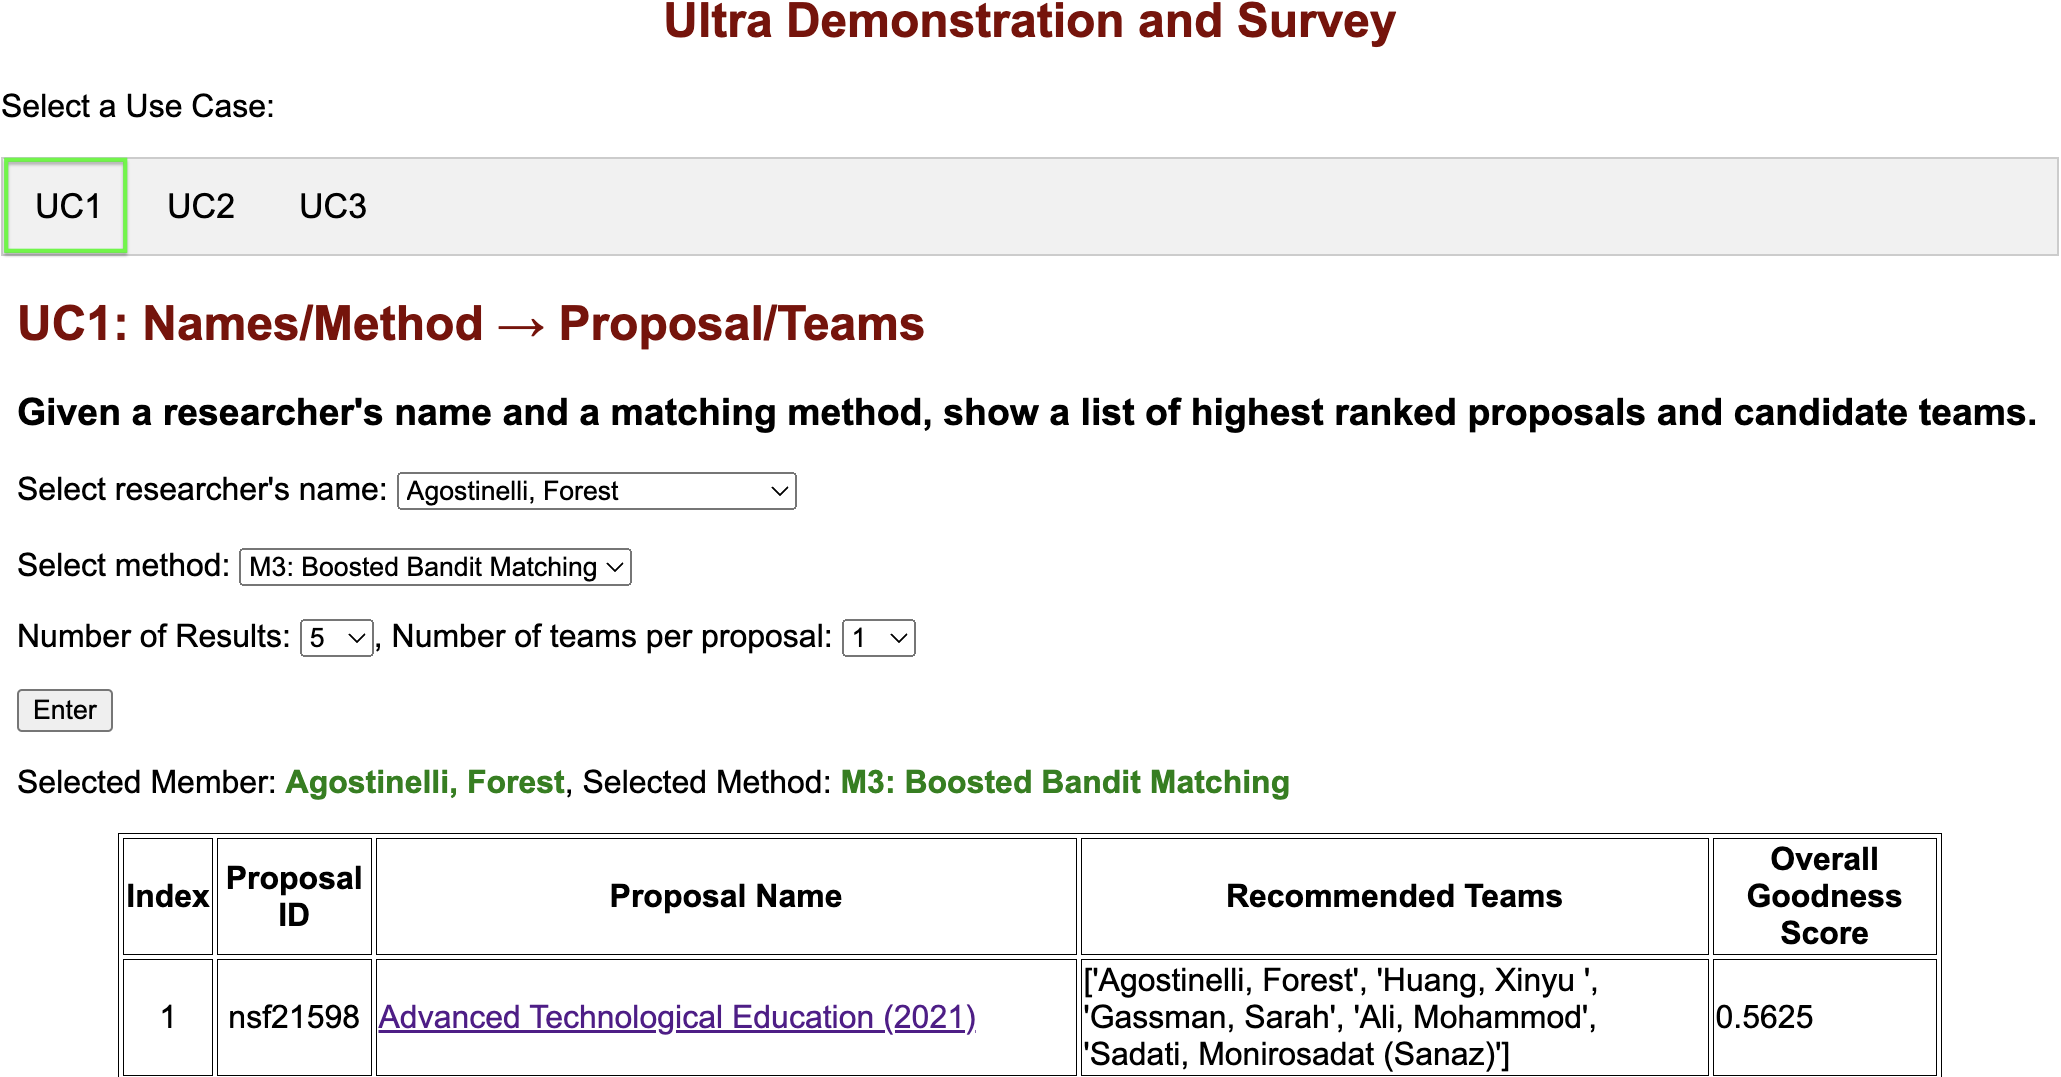
\includegraphics[width=1\linewidth]{figures/demo_uc1_larger_font.png}
    %{figures/demo_combined_image.png}
     %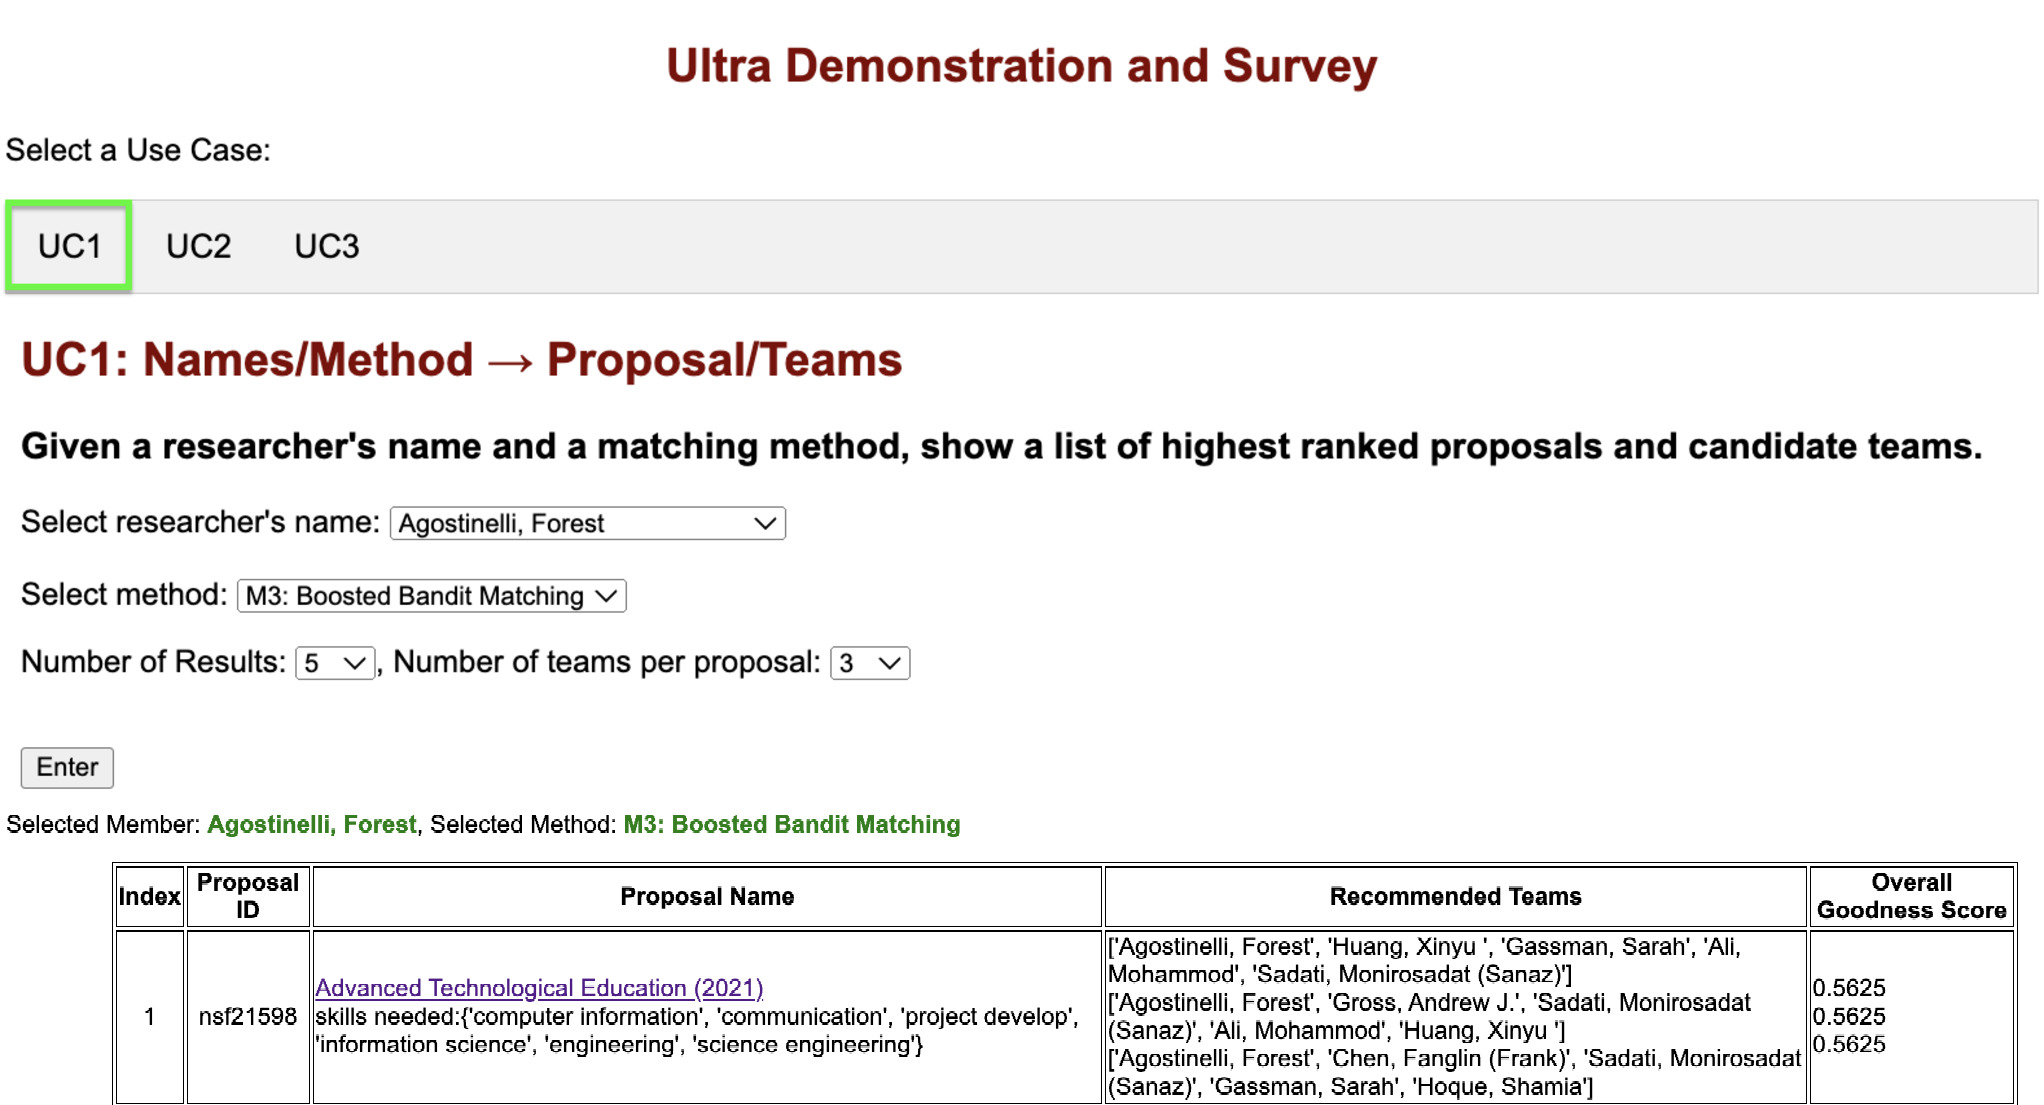
\includegraphics[scale=0.2]{figures/demo_combined_image.jpeg}
    \caption{A demo use case, ${UC}_1$, showing a team participant view of ULTRA.}
    \label{fig:ultra_system_usecases}
\end{figure}

We build upon prior work, ULTRA (\textbf{U}niversity-\textbf{L}ead \textbf{T}eam Builder from \textbf{R}FPs and \textbf{A}nalysis)~\cite{srivastava2022ultra}, a novel AI-based prototype for assisting with team formation when researchers respond to calls for proposals from funding agencies. In this paper, we interchangeably use the term \textit{call for proposal} with \textit{request for proposal (RFP).} 
Figure~\ref{fig:ultra_system_usecases} shows a demo\footnote{A full demo interaction with the ULTRA system can be found at https://www.youtube.com/watch?v=8MUtxsfVNIU. The tool is deployed at http://casy.cse.sc.edu/ultra/teaming/. Additional details about usecases, experiments, and survey resources are at \cite{ultra-resources}.} view of how the system works for an individual user who can become a team participant. 
The system first extracts technical skills from proposal calls found at publicly available data sources (e.g., NSF archives) and those present in online profiles of researchers (e.g., personal homepages, Google Scholar history), along with any additional teaming constraints that administrators or team participants of an institution may provide. Using AI and NLP techniques, ULTRA next provides a plausible list of candidate teams for each proposal call, where each team has at least two members. Our prior work~\cite{srivastava2022ultra}, however, is a use case of a {\em sequential} single-item recommendation problem, where solutions are often limited by known issues such as cold start~\cite{abdollahpouri2019managing} or popularity bias~\cite{yalcin2022evaluating}. Therefore, we expand on this work to include group recommendation and novel AI methods to recommend optimal teams. 
%The interested users in ULTRA are (1)~researchers looking for collaborative opportunities, and (2)~administrators at researchers’ organizations (e.g., university institutions) who want to promote more collaborations, proposals, and diversity at their institutions. 

Our contributions in the paper are that we:
\begin{itemize}
    \item formulate a novel {\em  group  recommendation problem} to  promote research collaborations where the objective is to suggest teams that could respond to calls for proposals, using skills found in open data, and balancing short- and long-term optimization.
    \item introduce a metric to measure goodness of teams and consider a configurable set of criteria: redundancy, group (set) size, coverage, and robustness.
    \item solve the novel problem using a variety of AI methods: string, taxonomy, and bandit (relational learning) methods, and compare them with a randomized baseline.
    \item  establish the benefit of the solution methods quantitatively using goodness metric. We find that more {\em informed methods lead to recommendations of smaller number of teams but higher goodness}.
    \item  establish the benefit of the system qualitatively using an IRB-approved preliminary survey at a College of a major US University. We find that {\em users broadly consider the tool useful as well as relevant} but more studies are needed. 
    \item demonstrate the generality of the approach with experiments at  two different institutions in US and India.  
    \item create and publish a teaming dataset that is available for research.

\end{itemize}